\documentclass[tikz, border=5mm]{standalone}
\usetikzlibrary{calc, arrows.meta, decorations.pathmorphing}

\begin{document}
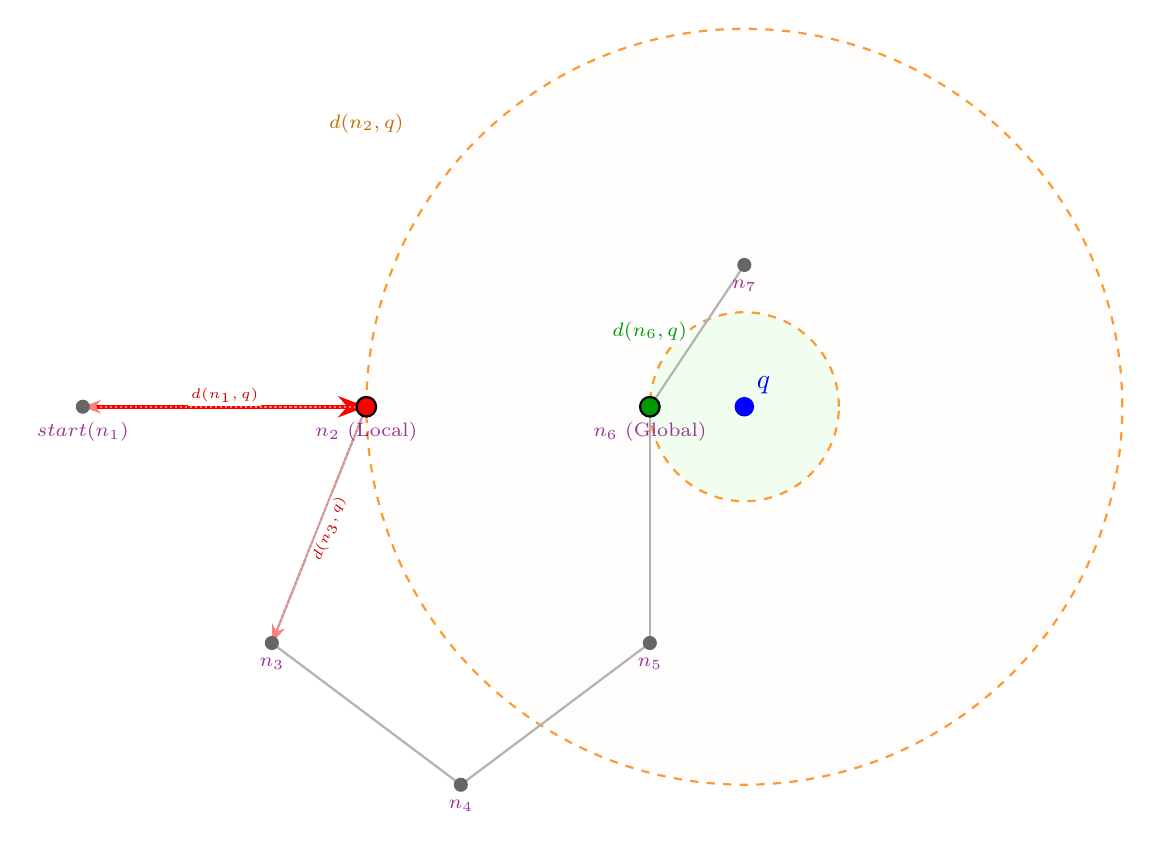
\begin{tikzpicture}[
    scale=1.2,
    % Estilos de nodos
    base node/.style={circle, fill=black!60, inner sep=1.8pt},
    query node/.style={circle, fill=blue, inner sep=2.5pt},
    local min/.style={circle, fill=red, inner sep=2.5pt, draw=black, thick},
    global min/.style={circle, fill=green!60!black, inner sep=2.5pt, draw=black, thick},
    node label/.style={below=2pt, font=\scriptsize, text=violet, opacity=0.8},
    % Estilos de aristas
    base edge/.style={thick, black!30},
    path edge/.style={->, >=Stealth, ultra thick, red},
    eval line/.style={densely dotted, thick, red!50},
    % Estilos de áreas y explicaciones
    distance circle/.style={dashed, thick, orange!80},
    text box/.style={fill=white, draw=black!20, rounded corners, font=\scriptsize, align=left, inner sep=4pt}
]

    % =========================================================================
    % 1. Definición de Coordenadas (Exactamente 7 nodos + q)
    % =========================================================================
    \coordinate (q) at (8, 5);

    % Nodos (1 a 7)
    \coordinate (n1) at (1, 5);   % start
    \coordinate (n2) at (4, 5);   % local_min
    \coordinate (n3) at (3, 2.5); % Puente inicio
    \coordinate (n4) at (5, 1);   % Fondo del puente
    \coordinate (n5) at (7, 2.5); % Puente subida
    \coordinate (n6) at (7, 5);   % global_min
    \coordinate (n7) at (8, 6.5); % Nodo extra para dar contexto al clúster destino

    % =========================================================================
    % 2. Isolíneas de Distancia desde q
    % =========================================================================
    % Circulo del Mínimo Local (Radio = distancia de q a n2 = 4)
    \draw[distance circle, fill=orange!5, fill opacity=0.3] (q) circle (4cm);
    \node[orange!80!black, font=\scriptsize, fill=white, inner sep=1pt] at (4, 8) {$d(n_2, q)$};

    % Circulo del Mínimo Global (Radio = distancia de q a n6 = 1)
    \draw[distance circle, fill=green!10, fill opacity=0.5] (q) circle (1cm);
    \node[green!60!black, font=\scriptsize, fill=white, inner sep=1pt] at (7, 5.8) {$d(n_6, q)$};

    % =========================================================================
    % 3. Aristas del Grafo (Ruta en U)
    % =========================================================================
    \draw[base edge] (n1) -- (n2);
    \draw[base edge] (n2) -- (n3);
    \draw[base edge] (n3) -- (n4);
    \draw[base edge] (n4) -- (n5);
    \draw[base edge] (n5) -- (n6);
    \draw[base edge] (n6) -- (n7);

    % =========================================================================
    % 5. Ejecución de la Búsqueda (Traza y Fallo)
    % =========================================================================
    % Ruta Greedy
    \draw[path edge] (n1) -- (n2);

    % Evaluación fallida: los únicos vecinos de n2 son n1 y n3, ambos están fuera del círculo
    \draw[eval line, ->, >=Stealth] (n2) -- (n3) node[midway, sloped, below, font=\tiny, text=red!80!black, fill=white, inner sep=1pt] {$d(n_3, q)$};
    \draw[eval line, ->, >=Stealth] (n2) -- (n1) node[midway, sloped, above, font=\tiny, text=red!80!black, fill=white, inner sep=1pt] {$d(n_1, q)$};

    % =========================================================================
    % 6. Dibujo de Nodos por encima de las líneas
    % =========================================================================
    \foreach \n in {n3, n4, n5, n7} {
        \node[base node] at (\n) {};
    }
    
    % Nodos Especiales
    \node[query node] at (q) {};
    \node[above right=1pt, font=\bfseries, blue] at (q) {$q$};
    
    \node[base node] at (n1) {};
    \node[local min] at (n2) {};
    \node[global min] at (n6) {};

    % Etiquetas Violetas
    \node[node label] at (n1) {$start (n_1)$};
    \node[node label] at (n2) {$n_2$ (Local)};
    \node[node label] at (n3) {$n_3$};
    \node[node label] at (n4) {$n_4$};
    \node[node label] at (n5) {$n_5$};
    \node[node label] at (n6) {$n_6$ (Global)};
    \node[node label] at (n7) {$n_7$};
\end{tikzpicture}
\end{document}

